%%
%% This is file `mcmthesis-demo.tex',
%% generated with the docstrip utility.
%%
%% The original source files were:
%%
%% mcmthesis.dtx  (with options: `demo')
%% !Mode:: "TeX:UTF-8"
%% -----------------------------------
%%
%% This is a generated file.
%%
%% Copyright (C)
%%     2010 -- 2015 by latexstudio
%%     2014 -- 2016 by Liam Huang
%%
%% This work may be distributed and/or modified under the
%% conditions of the LaTeX Project Public License, either version 1.3
%% of this license or (at your option) any later version.
%% The latest version of this license is in
%%   http://www.latex-project.org/lppl.txt
%% and version 1.3 or later is part of all distributions of LaTeX
%% version 2005/12/01 or later.
%%
%% This work has the LPPL maintenance status `maintained'.
%%
%% The Current Maintainer of this work is Liam Huang.
%%
\documentclass{mcmthesis}
\mcmsetup{CTeX = true,   % 使用 CTeX 套装时,设置为 true
        tcn = 0000, problem = B,
        sheet = true, titleinsheet = true, keywordsinsheet = true,
        titlepage = true, abstract = true}
\usepackage{palatino}
\usepackage{lipsum}
\title{The \LaTeX{} Template for MCM Version \MCMversion}
\author{\small \href{http://www.latexstudio.net/}
  {
\includegraphics[width=7cm]{mcmthesis-logo}}}
\date{\today}
\begin{document}



\section{Introduction}
\section{Assumptions}
\section{Model 1: T}
\subsection{Simulation and discussion}
.
.
.
\\
We simulate a toll plaze with 8 tollbooths and 3 lanes of travel.

Common vehicles are usually $4-4.5m$ long and $1.65-1.85m$ wide,
so a vehicle will take up 2 cells.
According to the \emph{Green Book, 1994}, an appropriate design of
a toll plaze would be a trapezoid with a
168-meter-long recovery zone and a 612-meter-long departure zone.
The width of a tollbooth along with a toll island
is usually $5.5m$, while that of each lane is $3.5-4m$.
We set the length of each cell equal to $2m$: $l_{car}=4m$.
So the parameters are as follows:
\[
{l}_{veh}=2\\
{w}_{veh}=1\\
WB={W}_{b}B=3\times8=24\\
WL={W}_{l}L=2\times3=6\\
{L}_{r}=84\\
{L}_{d}=306\\
\]

Figure~\ref{fig:q-p} shows the relationship between current throughput and
traffic flow density with different ${p}_{v}$.

%{翻译}当流量取得最大值q_max时对应的临界密度{d}_{c},zhegetu
%被临界midu划分为两部分,当流量小于临界密度dc时,车流为自由流.
%pv是随机减速概率,it varies between different drivers.figure shows that pv越小,对应的
%capacity 越大,dc也越大。在下面的章节里,我们主要采用了Pv=0.5来讨论,因为这时capacity约为700
%veh/h/lane,与实际情况个较为吻合

\begin{figure}[h]
\small
\centering
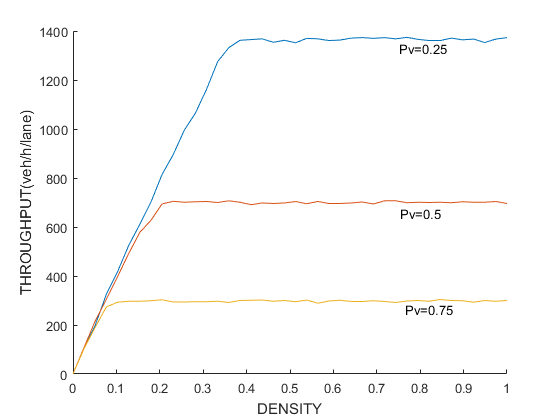
\includegraphics[width=12cm]{q-p-difPv.png}
\caption{The relationship between throughput and density with different ${p}_{v}$}
\label{fig:q-p}

\end{figure}

The density in the correspondence with the maximal throughput $q_{max}$ is
defined as critical density $d_{c}$. We can distinguish that the curves in
Figure~\ref{fig:q-p} are divided into two sections by that critical density.
If the flow density is lower than $d_{c}$, it will be a free flow; otherwise,
a crowded flow.

As mentioned above, ${p}_{v}$ is the probability of random deceleration.
It varies among different drivers. It is not difficult to conclude
that the smaller the value is, the larger $q_{max}$ is accessible. At the same
time, $d_{c}$ will increase correspondingly. In the following chapters, we
adopt ${p}_{v}=0.5$ as our basis, because the $q_{max}$ at this time is
consistent with the actual value, approximately $700 veh/h/lane$.





\end{document}

%%
%% This work consists of these files mcmthesis.dtx,
%%                                   figures/ and
%%                                   code/,
%% and the derived files             mcmthesis.cls,
%%                                   mcmthesis-demo.tex,
%%                                   README,
%%                                   LICENSE,
%%                                   mcmthesis.pdf and
%%                                   mcmthesis-demo.pdf.
%%
%% End of file `mcmthesis-demo.tex'.
